
\documentclass{article}
\usepackage[utf8]{inputenc}
\usepackage{tikz}

\begin{document}
\definecolor{c0000ff}{RGB}{0,0,255}


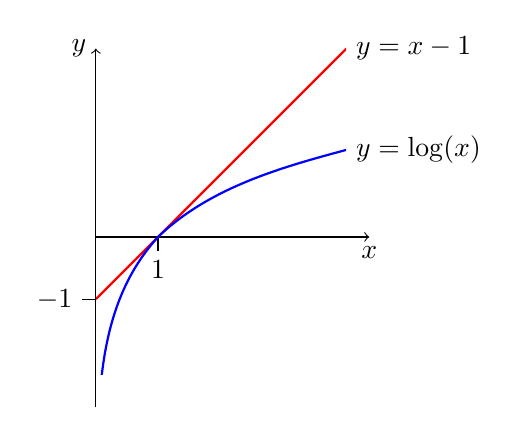
\begin{tikzpicture}[x=1.2pt,y=-1.2pt]
    \draw[->] (7.6680,58.7109) -- (90,58.7109) node[at end,below] {$x$};
    \draw[->] (7.6680,110) -- (7.6680,2) node[at end,left] {$y$};
    % 1x
    \draw (26.3828,58.7109) --++(270:5pt) node[below] {$1$};
    % 1y
    \draw (7.6680,77.6602)--++(180:5pt) node[left] {$-1$};
    \begin{scope}
        \clip (7.6680,100) rectangle (83,1);
        % line
        \path[draw=red,thick] (7.6680,77.4258) -- (83.1289,1.9648);
        % Log
        \path[draw=blue,thick] (7.6680,145.8398) .. controls (9.1414,116.2421) and (4.7208,82.2407) .. (26.5703,58.5234) .. controls (41.9458,43.9004) and (63.1458,37.8229) .. (83.1289,32.4846);
    \end{scope}
        \node[right] at (83.1289,1.9648) {$y=x-1$};
        \node[right] at (83.1289,32.4846) {$y=\log (x)$};
\end{tikzpicture}
\end{document}

